% AI4SE Workshop @ KI 2026 — Expanded Literature Review Draft
% Springer LNCS format — EXPANDED beyond 4 pages, to be condensed later
\documentclass[runningheads]{llncs}

\usepackage[T1]{fontenc}
\usepackage{graphicx}
\usepackage{hyperref}
\usepackage{microtype}
\usepackage{booktabs}
\usepackage{xcolor}
\usepackage{tikz}
\usepackage{pgfplots}
\pgfplotsset{compat=1.18}

\begin{document}

\title{Memory-Aware Software Engineering Agents:\\ Architectures, Mechanisms, and Open Gaps}

\titlerunning{Memory-Aware Software Engineering Agents}

\author{Michael Banf, Johannes Kuhn, Slawomir Garcarz \and Max Becker}

\authorrunning{Banf et al.}

\institute{Perelyn GmbH, Munich, Germany\\
\email{michael.banf@perelyn.com}}

\maketitle

\begin{abstract}
AI-assisted software engineering has progressed from code completion to
agentic systems operating across the full development lifecycle. Yet
these agents remain fundamentally stateless, i.e. each task begins without
memory of prior sessions, resolved bugs, or accumulated project
understanding. We present a survey that synthesizes
evidence from a feature-level
analysis of ten production software engineering harnesses with a specific focus on the current state of the art in memory architecture
for software engineering agents research. Our analysis reveals an episodic-temporal deficit, i.e. no production harness ships
episodic memory or temporal versioning natively. Interestingly, a rapidly growing
ecosystem of MCP-based memory add-ons has emerged to fill the
deficit. Yet, even these rarely implement temporal reasoning. Similarly, within the research community, while addressing episodic memory only a small fraction consider temporal
mechanisms. At the same time, benchmarks confirm a
factual-to-cognitive gap across production memory architectures. We argue that persistent, temporally grounded
memory is the prerequisite for software engineering agents that learn alongside the teams
they serve.

\keywords{Software Engineering Agents \and Agentic Memory \and
Context Engineering \and Temporal Reasoning \and Knowledge Graphs}
\end{abstract}

%%% ==================================================================
\section{Introduction}\label{sec:intro}
%%% ==================================================================

Agentic AI systems now operate across the full software engineering
lifecycle~\cite{becker2026,liu2024survey,jimenez2024swebench}. Whether
resolving complex bugs through multi-file analysis, discovering
architectural patterns, or coordinating code reviews across a team, these
agents accumulate significant task-specific knowledge during each
session. Yet that knowledge vanishes when the session ends: the next
invocation begins from scratch, repeating investigations, rediscovering
constraints, and re-learning project conventions.

The field has responded rapidly to the challenge~\cite{hu2025survey,memagents2026}, with every major AI provider now shipping
persistent memory. Interestingly, no production harness implements episodic memory or temporal
versioning natively, yet a thriving ecosystem of community-built MCP memory add-ons
has emerged, evidence that practitioners feel the deficit
acutely. However, fundamental properties such as temporal
versioning, team-shared memory, or decision provenance are only rarely addressed.

%%% ==================================================================
\section{Memory in Production Software Engineering Harnesses}\label{sec:harnesses}
%%% ==================================================================

The CoALA taxonomy~\cite{sumers2024} maps human memory types onto agent
components, i.e. \emph{working}, \emph{semantic}, i.e. conventions, facts, \emph{episodic}, such as past debugging experiences, and
\emph{procedural}, such as workflows or tool usage. Thereby, working memory is well-served by modern
context windows and semantic memory is partially addressed by context
files~\cite{agentreadmes2025}. However, episodic and procedural memory are almost
entirely absent. 

A finer-grained functional taxonomy~\cite{hu2025survey}
distinguishes \emph{factual}, i.e. what an agent knows, from \emph{experiential}, i.e. what the agent has learned from doing, and \emph{working} memory, i.e. active context management, with all three being critical for software engineering agents
operating over long project horizons. From this perspective, we analyzed the memory mechanisms of ten widely-used software engineering agent
harnesses. Table~\ref{tab:ecosystem} summarizes the
comparison across 20 dimensions grouped into six categories, i.e. CoALA memory types, 
memory operations, 
temporal mechanisms, 
software engineering specific capabilities, 
collaboration \& governance, and integration.

All ten harnesses support human-written instruction files, representing declarative semantic memory, with widespread adoption~\cite{agentreadmes2025}, yet little resolution improvement~\cite{gloaguen2026}. Context
engineering~\cite{contexteng2026} formalizes the approach, but all
implementations remain manually authored without temporal metadata. Five harnesses generate memories automatically (Claude Code, Codex CLI,
Copilot, Windsurf, Gemini CLI), but none distinguishes factual from
experiential knowledge. 
Context compaction triggers vary with respect to window utilization, however implementations are lossy, i.e.
technical details, intermediate reasoning steps, and
failed-approach information are discarded. However, the quality of compaction determines
whether memory helps or hinders~\cite{zhu2026}. 

No production system supports temporal versioning, i.e.\ tracking when
knowledge was valid, when it changed, or when it became stale. Neither do they support
episodic memory, i.e.\ structured records of past debugging sessions,
resolution trajectories, or decision rationale. Notably, those memory capabilities most critical for software engineering agents that
learn over time are those that no tool implements.

\begin{table}[h!]
\centering
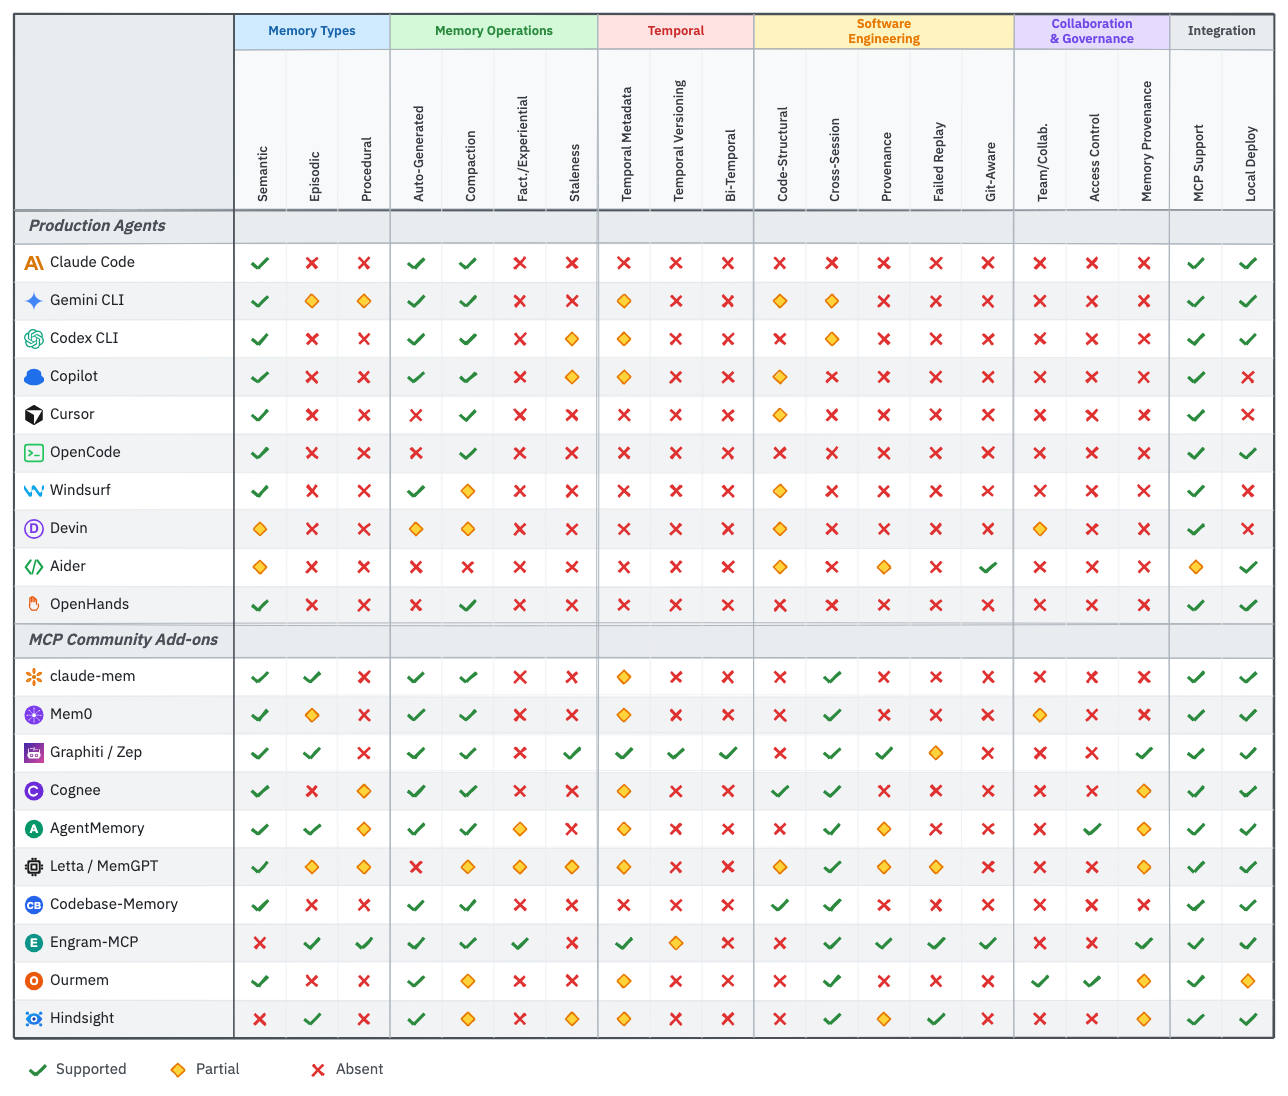
\includegraphics[width=\textwidth]{figures/ecosystem-table-expanded.png}
\caption{Memory capability matrix across 10 production SE agent harnesses and 10 representative MCP community add-ons, evaluated along 20 dimensions grouped into six categories: CoALA memory types, memory operations, temporal mechanisms, SE-specific capabilities, collaboration \& governance, and integration. Temporal versioning, bi-temporal validity, and governance remain near-universally absent.}
\label{tab:ecosystem}
\end{table}

\subsection{The community response: MCP memory add-ons}

The gap between what harnesses ship and what practitioners need has
spawned a rapidly growing ecosystem of community-built memory
extensions, primarily via the Model Context Protocol
(MCP)~\cite{mcpmemory2026}. Our survey identifies over 40 MCP-based
memory servers (see selection in table~\ref{tab:ecosystem}).
The ecosystem spans every CoALA memory type, however with stark
imbalances, i.e. semantic memory is near-universal,
episodic recall is emerging, while temporal versioning and procedural memory remain nearly absent. Among the most adopted, \emph{claude-mem}~\cite{claudemem2026} hooks into Claude Code lifecycle events for session
capture. \emph{AgentMemory}~\cite{agentmemory2026} provides hybrid of 
BM25 keyword search, vector embeddings and knowledge graph retrieval and
\emph{Graphiti/Zep}~\cite{rasmussen2025} remains the only reviewed
production system with true bi-temporal validity intervals.
Software engineering specific servers include
\emph{Codebase-Memory}~\cite{codebasemem2026}, a Tree-Sitter knowledge graph across
a plethora of languages, \emph{Engram-MCP}~\cite{engrammcp2026}, for git-branch-aware
session handoffs, or \emph{Hindsight}~\cite{hindsight2026}, featuring failed
attempt replay. Notably, nine of ten major coding agents now support MCP, making these add-ons agent-agnostic.
Built-in memory sophistication varies widely. For example, Gemini CLI
offers a four-tier hierarchy with automatic skills extraction, i.e. episodic-to-procedural conversion. Copilot performs just-in-time
codebase verification of stored facts, while Cursor has removed
its auto-memory feature, suggesting that naive auto-capture without
proper architecture degrades quality. 

%%% ==================================================================
\section{Memory Architectures: From Extraction to Graphs}\label{sec:architectures}
%%% ==================================================================

Our classification of the ICLR 2026 MemAgents workshop paper
collection~\cite{memagents2026} reveals that retrieval-augmented
memory is the dominant paradigm, underpinning over 60\% of
contributions. Within this paradigm, approaches differ primarily in
how they organize, consolidate, and temporally ground stored
memories. A second, smaller cluster of non-RAG approaches operates
at the model or inference level, including KV-cache compression,
attention-based, and embedding-based methods. Cross-cutting learning
strategies such as experience replay, reinforcement learning-based
management, and hierarchical consolidation span both clusters.
Three retrieval-augmented variants have reached production maturity
and been formally benchmarked head-to-head on the LoCoMo-Plus
cognitive memory evaluation~\cite{gurawaliya2026}, i.e. extraction-based, self-managing, and graph-based temporal. 

%%% ------------------------------------------------------------------
\subsection{Extraction-Based Memory}
%%% ------------------------------------------------------------------

Extraction-based architectures, such as Mem0~\cite{mem0_2025}, extract atomic facts from conversations and store
them as vector-indexed entries for similarity based querying. Extraction-based systems excel at
\emph{factual recall}. For software engineering tasks requiring explicit knowledge retrieval, this paradigm
is well-suited. However, extraction is lossy by design, e.g. the
process of converting debugging sessions into atomic facts discards
causal chains, temporal context, and reasoning paths~\cite{diagnosing2026}.

%%% ------------------------------------------------------------------
\subsection{Self-Managing Memory}
%%% ------------------------------------------------------------------

Self-Managing Memory, such as Letta~\cite{packer2023}, treats the LLM itself as an operating system
managing its own memory via explicit read/write/search operations over a
hierarchical store. The agent decides what to remember and how to
organize it. Self-managing memory excels at preserving
\emph{behavioral continuity}, i.e. reasoning on goals, recurring patterns, and evolving
state. For software engineering agents that must maintain an evolving picture of project
architecture, track long-running refactoring goals, or remember
what patterns emerged during debugging, this is the
strongest fit, although less transparent
than explicit stores: the agent's internal state cannot easily be
inspected, audited, or corrected by developers. 

\subsection{Graph-Based Temporal Memory}

Graph-Based temporal approaches, such as Graphiti~\cite{rasmussen2025}, can distinguish \emph{event time}, i.e. when
something happened, from \emph{ingestion time}, i.e. when the system learned
it, with every edge carrying explicit validity intervals. This
\emph{bi-temporal} approach is unique among production memory systems.
Graph-based memory excels at \emph{causal
reasoning}. For software engineering tasks requiring understanding of why a
decision was made, how events connect across time, or what caused a
regression, temporal graphs provide the most natural representation.
However, graph construction adds latency and complexity. 

%%% ------------------------------------------------------------------
\subsection{Hybrid and Emerging Approaches}
%%% ------------------------------------------------------------------
The LoCoMo-Plus results also make a compelling case for hybrid
architectures, since no single paradigm masters all competency
types~\cite{gurawaliya2026}, and it confirms that
the systems capture genuinely different aspects of the memory problem. To this end several emerging directions point toward future software engineering relevant
architectures. Reinforcement learning based memory management, such as Memory-R1~\cite{memoryr1_2025} and AgeMem~\cite{agemem2026} replace
heuristic memory policies with trained ones. The learned policies discover non-obvious strategies such as
preemptive summarization before the context window fills, suggesting a path toward adaptive memory management tuned
to software engineering specific reward signals such as issue resolution rate, code quality
metrics. Multi-graph memory, as in MAGMA~\cite{magma2026}, represents each memory item across orthogonal
semantic, temporal, causal, and entity graphs, with retrieval
formulated as policy-guided traversal. This decomposition offers
fine-grained control particularly relevant for software engineering: dependency
relationships via an entity graph, decision provenance via a causal graph,
API validity via a temporal graph, and conceptual similarity via a semantic
graph can be queried independently. A formal theory of hierarchical memory~\cite{hierarchicalmemory2026}
defines three operators, i.e. extraction, coarsening, and traversal. This identifies a
self-sufficiency spectrum for representative functions that
constrains viable retrieval strategies. TiMem~\cite{timem2026}
implements this via a temporal memory tree structure. For software engineering agents processing
long execution traces, hierarchical consolidation could be essential. Hybrid local/cloud architectures are also emerging: LightMem~\cite{lightmem2026} delegates memory operations, such as routing or
filtering, to small local models while reserving large models for
consolidation, and HyMem~\cite{hymem2026} achieves comparable
performance at reduced cost via dynamic two-tier retrieval.
Since the majority of MCP memory servers support fully local operation and
frameworks like Mem0, Letta, and Cognee run on Ollama, sovereign
deployments are feasible, though reliable MCP tool calling requires
14B+ parameter models~\cite{webcoach2026,erl2026}.

%%% ==================================================================
\section{Memory Mechanisms for Software Engineering}\label{sec:semechanisms}
%%% ==================================================================

Beyond general-purpose memory architectures, several mechanisms have
been developed specifically for or with direct relevance to software engineering agents.

%%% ------------------------------------------------------------------
\subsection{Versioned Context Management and Decision Provenance}
%%% ------------------------------------------------------------------

The Git Context Controller (GCC)~\cite{gcc2025} introduces Git-inspired
operations for agent memory, addressing the \emph{intra-session} memory
problem, i.e. managing working memory within a single task execution. The Lore protocol~\cite{lore2026} addresses the complementary
\emph{inter-session} problem as it repurposes git commit messages as
structured decision records carrying constraints, rejected alternatives,
agent directives, and verification metadata via native git trailers, introducing queryable decision provenance.
The practical need for decision provenance is acute. For example, each additional deviation in a
mutating action reduces success odds~\cite{saber2026}, with errors growing
as context length increases and agents drift from stale constraints, such as deprecated APIs~\cite{wang2025deprecated,ashik2026}.

%%% ------------------------------------------------------------------
\subsection{Experiential and Cross-Session Learning}
%%% ------------------------------------------------------------------

The SWE Context Bench~\cite{zhu2026} evaluates whether agents benefit from prior experience with one critical finding, i.e. summarized experience improves resolution, while unfiltered experience hurts. Experiential Co-Learning~\cite{qian2024} mines experiences from historical trajectories and injects them into future task
execution. Experiential Reflective Learning~\cite{erl2026} reflects on task trajectories to generate transferable
heuristics, i.e. actionable lessons that generalize across tasks. Live-SWE-agent~\cite{xia2025}, rather than remembering past experiences, self-creates
new tools during execution, representing procedural memory through self-modification. Structurally Aligned Subtask-Level Memory~\cite{subtaskmem2026} decomposes software engineering problem-solving into subtasks and aligns
memory storage and retrieval at the subtask rather than the whole-instance level. MemGrad~\cite{memgrad2026} transforms batches of behavioral feedback into
a dual memory strategy, i.e. retrospective memory captures recurring failure modes, while prospective memory encodes
gradient-derived strategies for future reasoning.  Procedural memory, such as Mem$^{\mathrm{p}}$~\cite{memp2025},
distills past agent trajectories into both
fine-grained step-by-step instructions and higher-level script-like
abstractions, creating learnable, updatable procedural memory.
Procedural knowledge built from a stronger model transfers effectively
to weaker ones. Strategy-level memory, such as ReasoningBank~\cite{reasoningbank2025},
rather than storing raw trajectories, distills
generalizable reasoning strategies from self-judged successes and
failures. Finally, persistent note-taking~\cite{cca2025} introduces a cross-session note-taking system where agents record
hindsight notes for compilation errors, runtime exceptions, and
unproductive strategies. WebCoach~\cite{webcoach2026} reveals a striking capacity threshold for experiential memory: 7B
models do not benefit from experiential memory, while 32B+ models
show pronounced gains. Self-generated
experiences outperform externally seeded ones~\cite{erl2026}. For software engineering agents, this implies that experiential
memory requires both sufficient model capacity to reason over retrieved
experience and careful curation to avoid context pollution.


%%% ------------------------------------------------------------------
\subsection{Knowledge Graphs for Software Engineering Agent Memory}
%%% ------------------------------------------------------------------

A comprehensive survey on graph-based agent memory~\cite{graphmemsurvey2026}
identifies four lifecycle phases, from extraction, that is converting raw data into graph nodes and edges, followed by
storage, i.e. organization and indexing, then retrieval, i.e.\ query-adaptive traversal,
and evolution, i.e. update, consolidate, forget. For software engineering agents, graph memory
offers three specific advantages. First, they naturally implement \emph{dependency tracking} via relationships for inherently graph-structured code
repositories, including files import modules,
classes inherit from others, functions call functions~\cite{codebasemem2026}. Second, they provide \emph{decision provenance}. Architectural decision
records, code review discussions, and commit rationale form a causal
graph of project decisions. Graph-based memory can model and preserve the
reasoning behind code structure, enabling agents to understand
constraints before proposing changes. Third, they lay a foundation for monitoring \emph{temporal evolution}.
For example, Graphiti's bi-temporal model maps naturally onto software evolution, such as an
invalid API, a recently adopted coding convention or deprecated dependency. GAM~\cite{gam2026} demonstrates the value of hierarchical graph
memory showing significant improvements over extraction-based
approaches by decoupling episodic from semantic consolidation via an
event progression graph. 

%%% ------------------------------------------------------------------
\subsection{Collaborative and Team Memory}\label{sec:collaborative}
%%% ------------------------------------------------------------------

Software engineering is inherently collaborative, yet memory research
exhibits a strong single-agent bias~\cite{memagents2026}. To this end, Collaborative Memory~\cite{rezazadeh2025} is the most
complete framework for multi-user memory sharing with dynamic access
control. It maintains two tiers. These are \emph{Private memory}, which is visible only to
the originating user and \emph{shared memory}, which consists of selectively shared
fragments, where each fragment carries immutable provenance attributes, i.e. contributing agents, accessed resources, timestamps. This architecture
maps naturally onto software engineering teams w.r.t private developer context, i.e. local
experiments, debugging notes, versus shared project knowledge, i.e. coding
conventions, architectural decisions, resolved issues. However, MINJA~\cite{minja2026} demonstrates that shared memory agents are vulnerable to query-only injection attacks. For software engineering
agents with access to codebases and deployment pipelines, memory
poisoning is a critical supply-chain risk. SSGM~\cite{ssgm2026} and MemArchitect~\cite{memarchitect2026} propose governance middleware for
evolving memory, while the mnemonic sovereignty survey~\cite{mnemonic2026}
addresses EU AI Act compliance. Yet no approach targets software engineering-specific governance
needs, such as access control aligned with repository permissions, memory
provenance linked to code review approvals, or temporal policies tied
to release cycles.


%%% ==================================================================
\section{Discussion: Open Gaps}\label{sec:gaps}
%%% ==================================================================

Synthesizing our analysis, we identified several open gaps specific to memory
for software engineering agents as inspirations for future research. Software engineering agents discard resolution trajectories after each session. Early
research solutions exist, but no production
harness or community add-on integrates cross-session learning. No production software engineering agent and only a tiny fraction of community add-ons track temporal knowledge validity.
No software engineering specific
temporal memory exists. Also, there exists only one software engineering specific temporal
benchmark. Convention retention, experience transfer,
staleness detection, and decision provenance remain unevaluated. Collaborative memory is rarely addressed, yet software engineering teams
need shared decisions, private debugging notes, and repository-aligned
access control. Research on memory injection attacks demonstrates that shared-memory agents lack adequate governance and security, while GDPR-compliant deletion remains entirely unaddressed. Software engineering craft knowledge is overwhelmingly procedural, yet procedural memory
is the rarest type in both research and the community
ecosystem. The MCP ecosystem provides a composable memory architecture where
each server addresses a different CoALA memory type. Yet no orchestration layer decides which
memory to consult when, resolves conflicts between overlapping stores,
or manages lifecycle across layers. Assembling the full stack remains
a manual integration challenge. Closing these gaps will require a
coordinated effort and a clear vision of transforming software engineering agents from amnesic
tools into learning collaborators that grow alongside the
software they help build.

%%% ==================================================================
\begin{thebibliography}{50}
\scriptsize
\setlength{\itemsep}{-1pt}
\setlength{\parsep}{0pt}

\bibitem{becker2026}
Becker, M.: Der KI-gest\"utzte Software-Entwicklungsprozess. BVMW, Perelyn GmbH (2026)

\bibitem{liu2024survey}
Liu, J., et al.: LLM-Based Agents for SE: A Survey. ACM TOSEM (2024)

\bibitem{jimenez2024swebench}
Jimenez, C.E., et al.: SWE-bench: Can LMs Resolve Real-World GitHub Issues? ICLR (2024)

\bibitem{sumers2024}
Sumers, T.R., et al.: Cognitive Architectures for Language Agents. TMLR (2024)

\bibitem{hu2025survey}
Hu, Y., et al.: Memory in the Age of AI Agents: A Survey. arXiv:2512.13564 (2025)

\bibitem{memagents2026}
MemAgents: Memory for LLM-Based Agentic Systems. ICLR 2026 Workshop

\bibitem{agentreadmes2025}
Chatlatanagulchai, W., et al.: Agent READMEs: Context Files for Agentic Coding. arXiv:2511.12884 (2025)

\bibitem{gloaguen2026}
Gloaguen, J., et al.: Evaluating AGENTS.md. MemAgents@ICLR (2026)

\bibitem{gurawaliya2026}
Gurawaliya, H., et al.: Agentic Memory Realized. appliedAI Initiative (2026)

\bibitem{mem0_2025}
Chhikara, P., et al.: Mem0: Production-Ready Long-Term Memory. ECAI (2025)

\bibitem{packer2023}
Packer, C., et al.: MemGPT: Towards LLMs as Operating Systems. arXiv:2310.08560 (2023)

\bibitem{rasmussen2025}
Rasmussen, P., et al.: Zep: Temporal KG for Agent Memory. arXiv:2501.13956 (2025)

\bibitem{diagnosing2026}
Diagnosing Retrieval vs.\ Utilization Bottlenecks in Agent Memory. MemAgents@ICLR (2026)

\bibitem{gcc2025}
Wu, J., et al.: Git Context Controller. arXiv:2508.00031 (2025)

\bibitem{lore2026}
Stetsenko, I.: Lore: Git Commits as Structured Knowledge Protocol. arXiv:2603.15566 (2026)

\bibitem{qian2024}
Qian, C., et al.: Experiential Co-Learning of Software-Developing Agents. ACL (2024)

\bibitem{erl2026}
ERL: Experiential Reflective Learning for Self-Improving LLM Agents. MemAgents@ICLR (2026)

\bibitem{xia2025}
Xia, C.S., et al.: Live-SWE-agent: Can SE Agents Self-Evolve? arXiv:2511.13646 (2025)

\bibitem{subtaskmem2026}
Subtask-Level Memory for SE Agents. arXiv:2602.21611 (2026)

\bibitem{memgrad2026}
Natekar, P., et al.: MemGrad: Memory-Guided Agentic SE Optimization. MemAgents@ICLR (2026)

\bibitem{zhu2026}
Zhu, J., et al.: SWE Context Bench. arXiv:2602.08316 (2026)

\bibitem{graphmemsurvey2026}
Yang, C., et al.: Graph-based Agent Memory: A Survey. arXiv:2602.05665 (2026)

\bibitem{magma2026}
MAGMA: Multi-Graph Agentic Memory Architecture. arXiv:2601.03236 (2026)

\bibitem{timem2026}
TiMem: Temporal-Hierarchical Memory Consolidation. arXiv:2601.02845 (2026)

\bibitem{gam2026}
Wu, Z., et al.: GAM: Hierarchical Graph Memory for Agents. ICLR (2026)

\bibitem{memoryr1_2025}
Memory-R1: RL Framework with Memory Manager. arXiv (2025)

\bibitem{agemem2026}
AgeMem: Agentic Memory with Unified LTM/STM via RL. arXiv (2026)

\bibitem{wang2025deprecated}
Wang, C., et al.: Deprecated API Usage in LLM Code Completion. ICSE (2025)

\bibitem{ashik2026}
Ashik, A.N., et al.: Knowledge Conflicts from Evolving APIs. arXiv:2604.09515 (2026)

\bibitem{saber2026}
SABER: Safeguarding Mutating Steps in LLM Agents. MemAgents@ICLR (2026)

\bibitem{rezazadeh2025}
Rezazadeh, A., et al.: Collaborative Memory for LLM Agents. arXiv:2505.18279 (2025)

\bibitem{minja2026}
Zeng, H., et al.: MINJA: Memory Injection Attacks on Agents. MemAgents@ICLR (2026)

\bibitem{ssgm2026}
Lam, C., et al.: SSGM: Governing Evolving Memory. arXiv:2603.11768 (2026)

\bibitem{memarchitect2026}
Kumar, L.S., et al.: MemArchitect: Policy-Driven Memory Governance. arXiv:2603.18330 (2026)

\bibitem{webcoach2026}
WebCoach: Self-Evolving Web Agents with Cross-Session Memory. MemAgents@ICLR (2026)

\bibitem{codebasemem2026}
Vogel, M., et al.: Codebase-Memory: Tree-Sitter KG via MCP. arXiv:2603.27277 (2026)

\bibitem{memp2025}
Fang, R., et al.: Mem$^{\mathrm{p}}$: Agent Procedural Memory. arXiv:2508.06433 (2025)

\bibitem{mcpmemory2026}
Anthropic: Model Context Protocol. \url{https://modelcontextprotocol.io} (2026)

\bibitem{agentmemory2026}
agentmemory: Persistent Memory MCP Server. GitHub (2026)

\bibitem{claudemem2026}
claude-mem: Lifecycle-Hook Memory for Coding Agents. GitHub (2026)

\bibitem{engrammcp2026}
edg-l: Engram-MCP --- Git Branch-Aware Session Handoffs. GitHub (2026)

\bibitem{hindsight2026}
Shazil, S.: Hindsight --- Attempt Memory for Coding Agents. GitHub (2026)

\bibitem{lightmem2026}
LightMem: SLMs for Online Memory Management. arXiv:2604.07798 (2026)

\bibitem{hymem2026}
HyMem: Dynamic Dual-Granular Retrieval. arXiv:2602.13933 (2026)

\bibitem{contexteng2026}
Willison, S.: Context Engineering. simonwillison.net (2025)

\bibitem{hierarchicalmemory2026}
Talebirad, Y., et al.: Toward a Theory of Hierarchical Memory for Language Agents. ICLR (2026)

\bibitem{reasoningbank2025}
Ouyang, S., et al.: ReasoningBank: Scaling Agent Self-Evolving with Reasoning Memory. arXiv:2509.25140 (2025)

\bibitem{cca2025}
Wong, S., et al.: Confucius Code Agent: Scalable Scaffolding for Real-World Codebases. arXiv:2512.10398 (2025)

\bibitem{mnemonic2026}
Security of Long-Term Memory in LLM Agents: Toward Mnemonic Sovereignty. arXiv:2604.16548 (2026)

\end{thebibliography}

\end{document}
